\documentclass[aspectratio=169, 11pt]{beamer}

% ── Theme & Colors ──────────────────────────────────────────────────
\usetheme{Madrid}
\usecolortheme{whale}
\definecolor{navy}{RGB}{0,31,91}
\definecolor{accent}{RGB}{0,119,182}
\definecolor{good}{RGB}{39,174,96}
\definecolor{bad}{RGB}{231,76,60}
\setbeamercolor{title}{fg=white,bg=navy}
\setbeamercolor{frametitle}{fg=white,bg=navy}
\setbeamercolor{structure}{fg=navy}
\setbeamercolor{block title}{bg=accent,fg=white}
\setbeamercolor{block body}{bg=accent!10}
\setbeamertemplate{navigation symbols}{}
\setbeamertemplate{footline}[frame number]

% ── Packages ────────────────────────────────────────────────────────
\usepackage{booktabs}
\usepackage{graphicx}
\usepackage{amsmath,amssymb}
\usepackage{tikz}
\usepackage{colortbl}
\usepackage{multirow}
\usepackage{adjustbox}
\usepackage{xcolor}
\usepackage{fontawesome5}

\graphicspath{{results/plots/}}

\newcommand{\up}[1]{\textcolor{good}{\textbf{+#1}}}
\newcommand{\down}[1]{\textcolor{bad}{\textbf{#1}}}
\newcommand{\tie}[1]{\textcolor{gray}{\textbf{#1}}}

% ════════════════════════════════════════════════════════════════════
\title[Foundation Model for PHM]{A Self-Supervised Foundation Model\\for Industrial Health Monitoring}
\subtitle{Cross-Domain Pre-Training with Masked Autoencoders\\for Prognostics and Health Management}
\author{Zaynab Raounak}
\date{\today}

\begin{document}

% ════════════════════════════════════════════════════════════════════
%  TITLE
% ════════════════════════════════════════════════════════════════════
\begin{frame}
\titlepage
\end{frame}

% ════════════════════════════════════════════════════════════════════
%  OUTLINE
% ════════════════════════════════════════════════════════════════════
\begin{frame}{Outline}
\tableofcontents
\end{frame}

% ════════════════════════════════════════════════════════════════════
\section{Motivation}
% ════════════════════════════════════════════════════════════════════

\begin{frame}{Why a Foundation Model for PHM?}
\begin{columns}[T]
\begin{column}{0.52\textwidth}
\textbf{The Problem}
\begin{itemize}
    \item Industrial equipment generates \textbf{massive unlabeled} vibration/sensor data
    \item Labeled fault data is \textbf{scarce and expensive}---failures are rare events
    \item Existing models are \textbf{domain-specific}: a bearing model cannot diagnose gears
    \item Deploying a new model per machine type is \textbf{not scalable}
\end{itemize}
\end{column}
\begin{column}{0.45\textwidth}
\textbf{Our Hypothesis}
\begin{block}{Foundation Model Advantage}
A single self-supervised model pre-trained across \textbf{multiple industrial domains} can:
\begin{enumerate}
    \item Match or exceed supervised baselines
    \item Excel in \textbf{low-data regimes} (few-shot)
    \item \textbf{Transfer across domains} zero-shot
\end{enumerate}
\end{block}
\end{column}
\end{columns}
\end{frame}

% ════════════════════════════════════════════════════════════════════
\section{Datasets}
% ════════════════════════════════════════════════════════════════════

\begin{frame}{Five Industrial Domains}
\begin{table}
\centering
\small
\begin{tabular}{@{}lllrl@{}}
\toprule
\textbf{Dataset} & \textbf{Equipment} & \textbf{Task} & \textbf{Freq (Hz)} & \textbf{Classes / Target} \\
\midrule
CWRU      & Bearing (drive end)   & Classification & 12\,000   & 4 fault types \\
PRONOSTIA & Bearing (run-to-fail) & RUL Regression & 25\,600   & Remaining life \\
CMAPSS    & Turbofan engine       & RUL Regression & 1 (cycle) & Remaining life \\
MFPT      & Bearing               & Classification & 97\,656   & 2 (normal/fault) \\
UOC18     & Gearbox               & Classification & 20\,000   & 9 operating cond. \\
\bottomrule
\end{tabular}
\end{table}

\vspace{0.4cm}
\begin{block}{Key Challenge: Heterogeneous Sampling Rates}
Frequencies span \textbf{5 orders of magnitude} (1\,Hz to 97\,kHz).\\
Our architecture handles this via \textbf{Frequency-Conditioned Layer Normalization}.
\end{block}
\end{frame}

% ════════════════════════════════════════════════════════════════════
\section{Architecture}
% ════════════════════════════════════════════════════════════════════

\begin{frame}{Model Architecture Overview}
\begin{center}
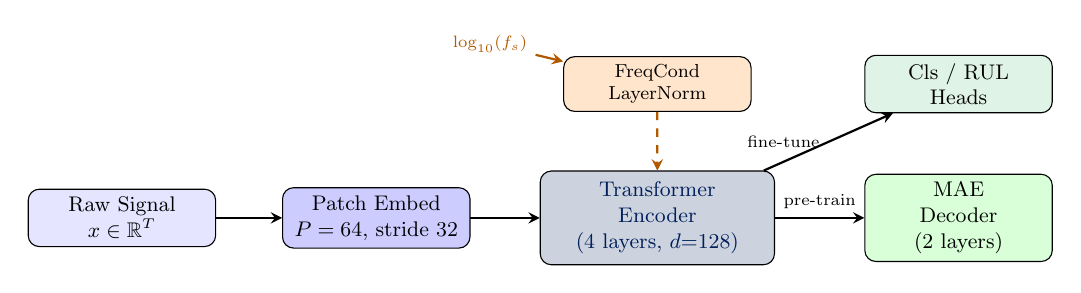
\begin{tikzpicture}[
    box/.style={draw, rounded corners, minimum width=2.8cm, minimum height=0.8cm, align=center, font=\small},
    arr/.style={->, thick, >=stealth},
    scale=0.85, transform shape
]
% Input
\node[box, fill=blue!10] (input) at (0,0) {Raw Signal\\$x \in \mathbb{R}^{T}$};
% Patcher
\node[box, fill=blue!20] (patch) at (3.8,0) {Patch Embed\\$P=64$, stride $32$};
% Encoder
\node[box, fill=navy!20, text=navy, minimum width=3.5cm, minimum height=1.4cm] (enc) at (8,0) {Transformer\\Encoder\\(4 layers, $d{=}128$)};
% FreqCond
\node[box, fill=orange!20, font=\footnotesize] (freq) at (8,2) {FreqCond\\LayerNorm};
% Decoder
\node[box, fill=green!15] (dec) at (12.5,0) {MAE\\Decoder\\(2 layers)};
% Heads
\node[box, fill=good!15] (cls) at (12.5,2) {Cls / RUL\\Heads};

\draw[arr] (input) -- (patch);
\draw[arr] (patch) -- (enc);
\draw[arr, dashed, orange!70!black] (freq) -- (enc);
\draw[arr] (enc) -- (dec) node[midway, above, font=\scriptsize] {pre-train};
\draw[arr] (enc) -- (cls) node[midway, left, font=\scriptsize] {fine-tune};

% Sampling freq input
\node[font=\scriptsize, orange!70!black] (fs) at (5.5,2.6) {$\log_{10}(f_s)$};
\draw[arr, orange!70!black] (fs) -- (freq);
\end{tikzpicture}
\end{center}

\vspace{0.3cm}
\begin{columns}[T]
\begin{column}{0.48\textwidth}
\textbf{Encoder:} 4-layer Transformer, $d_\text{model}=128$, 4 heads, channel-independent (PatchTST-style)
\end{column}
\begin{column}{0.48\textwidth}
\textbf{Decoder:} 2-layer lightweight Transformer for masked patch reconstruction (discarded after pre-training)
\end{column}
\end{columns}
\end{frame}

% ────────────────────────────────────────────────────────────────────

\begin{frame}{Frequency-Conditioned Layer Normalization}

\textbf{Problem:} Datasets span 1\,Hz -- 97\,kHz. Standard normalization cannot adapt to such diverse temporal scales.

\vspace{0.3cm}
\textbf{Solution:} FiLM-style conditioning on the sampling frequency.

\[
\text{FreqCondNorm}(h) = \gamma(f_s) \cdot \frac{h - \mu}{\sigma} + \beta(f_s)
\]

where $\gamma, \beta = \text{MLP}\bigl(\log_{10}(f_s)\bigr)$ are learned affine parameters.

\vspace{0.3cm}
\begin{block}{Why This Matters}
\begin{itemize}
    \item Each Transformer layer adapts its normalization statistics to the signal's native frequency
    \item A 1\,Hz turbofan signal and a 97\,kHz vibration signal are processed by the \textbf{same weights} but with frequency-appropriate normalization
    \item This is our \textbf{key architectural contribution} enabling true multi-domain pre-training
\end{itemize}
\end{block}
\end{frame}

% ════════════════════════════════════════════════════════════════════
\section{Pre-Training: Masked Autoencoder}
% ════════════════════════════════════════════════════════════════════

\begin{frame}{Self-Supervised Pre-Training with MAE}
\begin{columns}[T]
\begin{column}{0.55\textwidth}
\textbf{Masked Autoencoder (He et al., CVPR 2022)}
\begin{enumerate}
    \item Divide signal into patches ($P{=}64$, stride $32$)
    \item Randomly mask \textbf{50\%} of patches
    \item Encoder processes \textbf{only visible patches} (efficiency + forces learning)
    \item Insert learnable mask tokens
    \item Decoder reconstructs \textbf{masked patches}
\end{enumerate}

\vspace{0.3cm}
\textbf{Loss:} MSE on masked patches only, with \textbf{patch-level normalization} (zero mean, unit variance per patch)

\[
\mathcal{L} = \frac{1}{|\mathcal{M}|}\sum_{i \in \mathcal{M}} \| \hat{p}_i - \tilde{p}_i \|^2
\]
\end{column}
\begin{column}{0.42\textwidth}
\textbf{Training Details}
\begin{itemize}
    \item 200 epochs, batch size 256
    \item AdamW, LR $10^{-4}$
    \item Warmup + cosine annealing
    \item Patience 30 (early stopping)
\end{itemize}

\vspace{0.3cm}
\textbf{Pre-Training Data}\\
All 5 datasets combined (\textbf{unlabeled})---the model never sees fault labels during pre-training.

\vspace{0.3cm}
\textbf{Key Design Choice}\\
True MAE: encoder sees \textbf{only 50\%} of tokens $\Rightarrow$ cannot ``cheat'' by interpolating from neighbors.
\end{column}
\end{columns}
\end{frame}

% ────────────────────────────────────────────────────────────────────

\begin{frame}{Pre-Training Convergence}
\begin{columns}[T]
\begin{column}{0.55\textwidth}
\begin{figure}
    \centering
    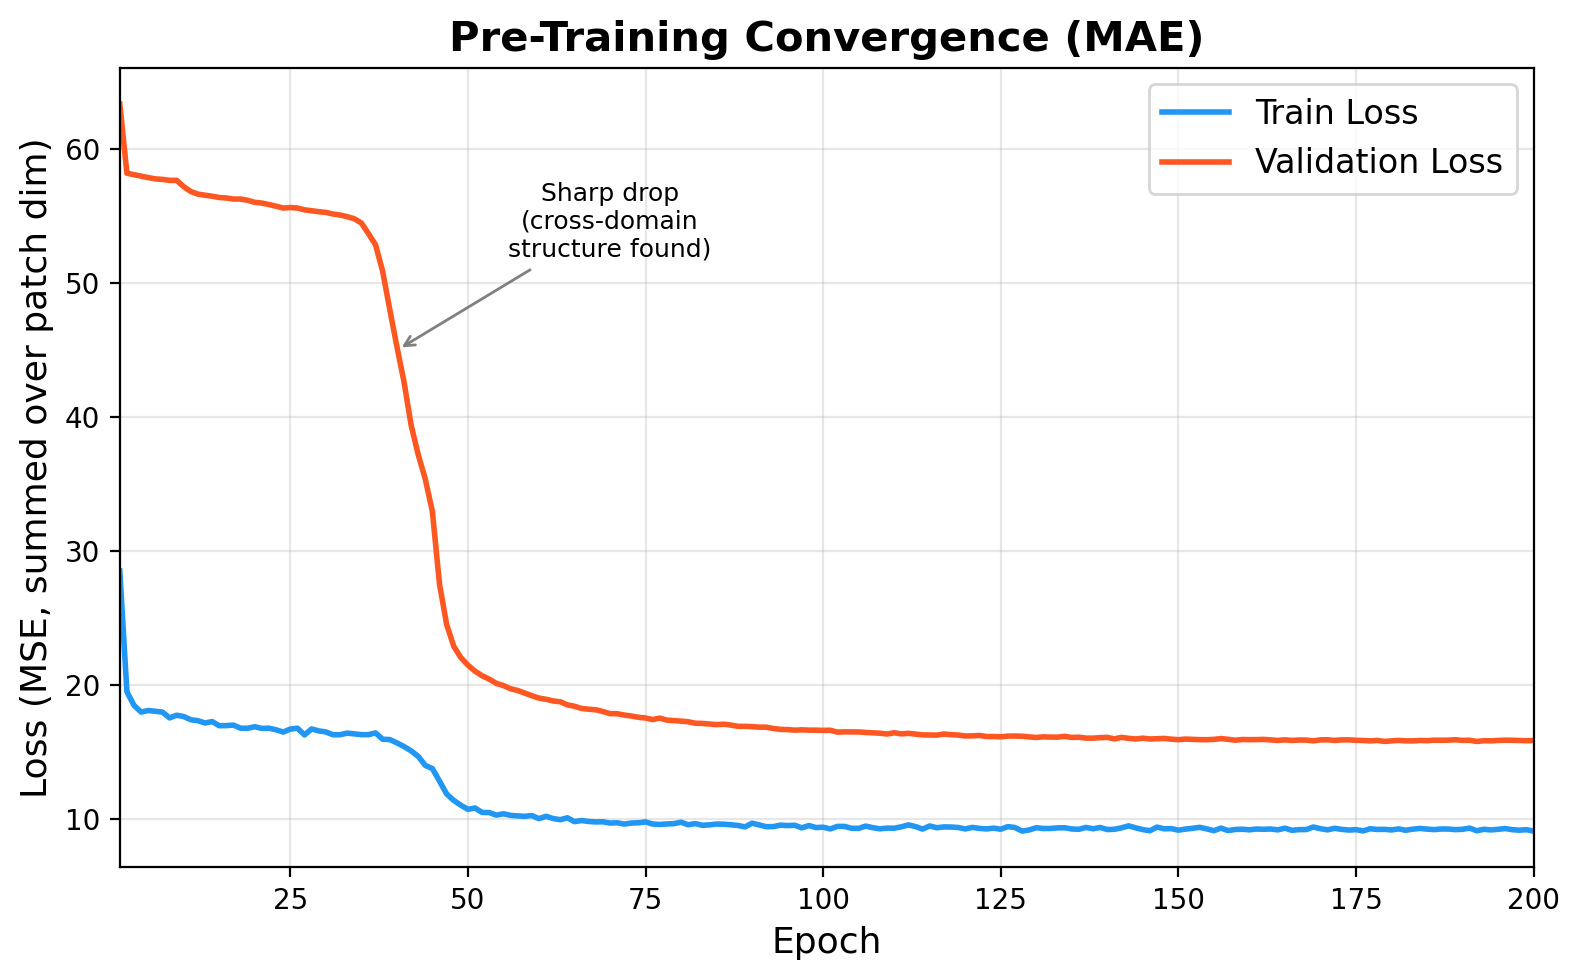
\includegraphics[width=\linewidth]{pretrain_loss.png}
    \caption*{Training and validation loss over 200 epochs.}
\end{figure}
\end{column}
\begin{column}{0.42\textwidth}
\textbf{Convergence Summary}
\begin{itemize}
    \item Train loss: $28.5 \rightarrow 9.1$ \quad (68\% $\downarrow$)
    \item Val loss: $63.4 \rightarrow 15.8$ \quad (75\% $\downarrow$)
    \item Sharp drop at epoch ${\sim}38$: model discovers cross-domain structure
    \item Smooth convergence after epoch 100
\end{itemize}

\vspace{0.3cm}
\begin{block}{Per-Element MSE}
Reported loss is summed over patch dim ($P{=}64$).\\
Actual per-element MSE: $9.1 / 64 = \mathbf{0.14}$\\
(normalized target $\sim\mathcal{N}(0,1)$, so 0.14 is excellent)
\end{block}
\end{column}
\end{columns}
\end{frame}

% ════════════════════════════════════════════════════════════════════
\section{Fine-Tuning Strategy}
% ════════════════════════════════════════════════════════════════════

\begin{frame}{3-Stage Progressive Fine-Tuning}
\begin{center}
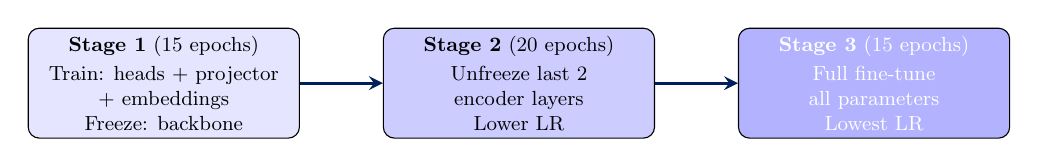
\begin{tikzpicture}[
    stage/.style={draw, rounded corners, minimum width=4.2cm, minimum height=1.6cm, align=center, font=\small},
    arr/.style={->, very thick, >=stealth, navy},
    scale=0.82, transform shape
]
\node[stage, fill=blue!10] (s1) at (0,0) {\textbf{Stage 1} (15 epochs)\\[2pt] Train: heads + projector\\+ embeddings\\Freeze: backbone};
\node[stage, fill=blue!20] (s2) at (5.5,0) {\textbf{Stage 2} (20 epochs)\\[2pt] Unfreeze last 2\\encoder layers\\Lower LR};
\node[stage, fill=blue!30, text=white] (s3) at (11,0) {\textbf{Stage 3} (15 epochs)\\[2pt] Full fine-tune\\all parameters\\Lowest LR};

\draw[arr] (s1) -- (s2);
\draw[arr] (s2) -- (s3);
\end{tikzpicture}
\end{center}

\vspace{0.4cm}
\textbf{Rationale:}
\begin{itemize}
    \item \textbf{Stage 1:} Align the randomly initialized task heads to the pre-trained feature space without corrupting the backbone
    \item \textbf{Stage 2:} Allow the top encoder layers to adapt domain-specific features
    \item \textbf{Stage 3:} End-to-end refinement with small LR to squeeze out final performance
\end{itemize}

\vspace{0.2cm}
\textit{Baseline CNN is trained from scratch with the same total epoch budget for fair comparison.}
\end{frame}

% ════════════════════════════════════════════════════════════════════
\section{Results: Full-Data Evaluation}
% ════════════════════════════════════════════════════════════════════

\begin{frame}{Classification: Accuracy Comparison}
\begin{columns}[T]
\begin{column}{0.52\textwidth}
\begin{figure}
    \centering
    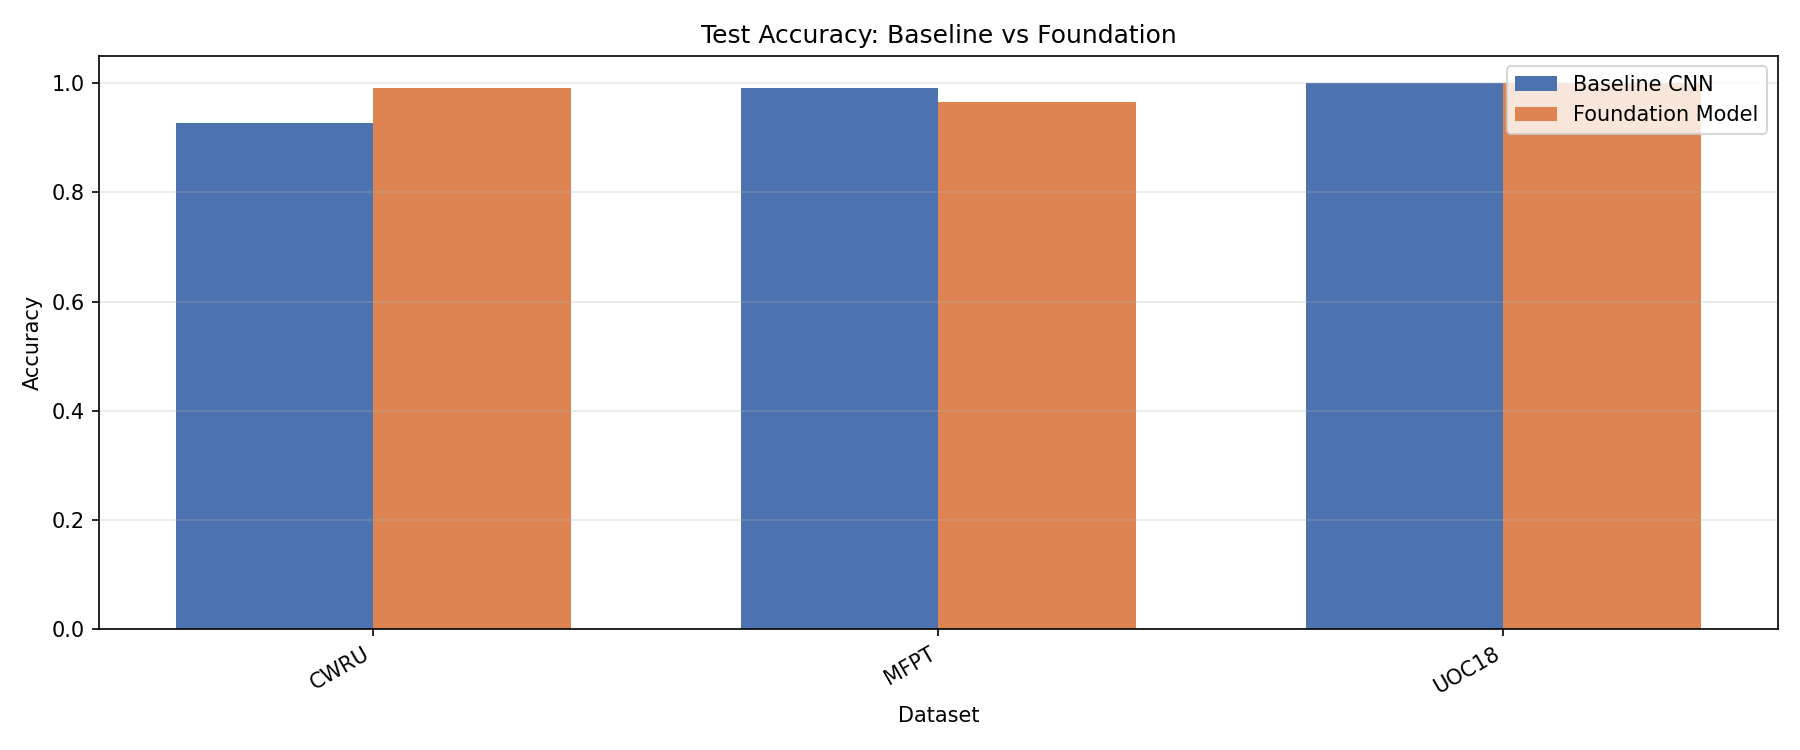
\includegraphics[width=\linewidth]{accuracy_comparison.png}
\end{figure}
\end{column}
\begin{column}{0.45\textwidth}
\begin{table}
\centering
\small
\begin{tabular}{@{}lccl@{}}
\toprule
\textbf{Dataset} & \textbf{Base} & \textbf{Found.} & \textbf{$\Delta$} \\
\midrule
CWRU  & 92.8\% & \textbf{99.2\%} & \up{6.4\%} \\
MFPT  & \textbf{99.2\%} & 96.6\% & \down{$-$2.6\%} \\
UOC18 & \textbf{100\%} & \textbf{100\%} & \tie{0.0\%} \\
\bottomrule
\end{tabular}
\end{table}

\vspace{0.3cm}
\begin{itemize}
    \item \textbf{CWRU:} Foundation achieves near-perfect 99.2\%, a significant +6.4\% gain
    \item \textbf{UOC18:} Both achieve 100\%---dataset may be ``solved''
    \item \textbf{MFPT:} Small dataset (117 samples); baseline overfits more effectively here
\end{itemize}
\end{column}
\end{columns}
\end{frame}

% ────────────────────────────────────────────────────────────────────

\begin{frame}{Classification: F1 Score Comparison}
\begin{columns}[T]
\begin{column}{0.52\textwidth}
\begin{figure}
    \centering
    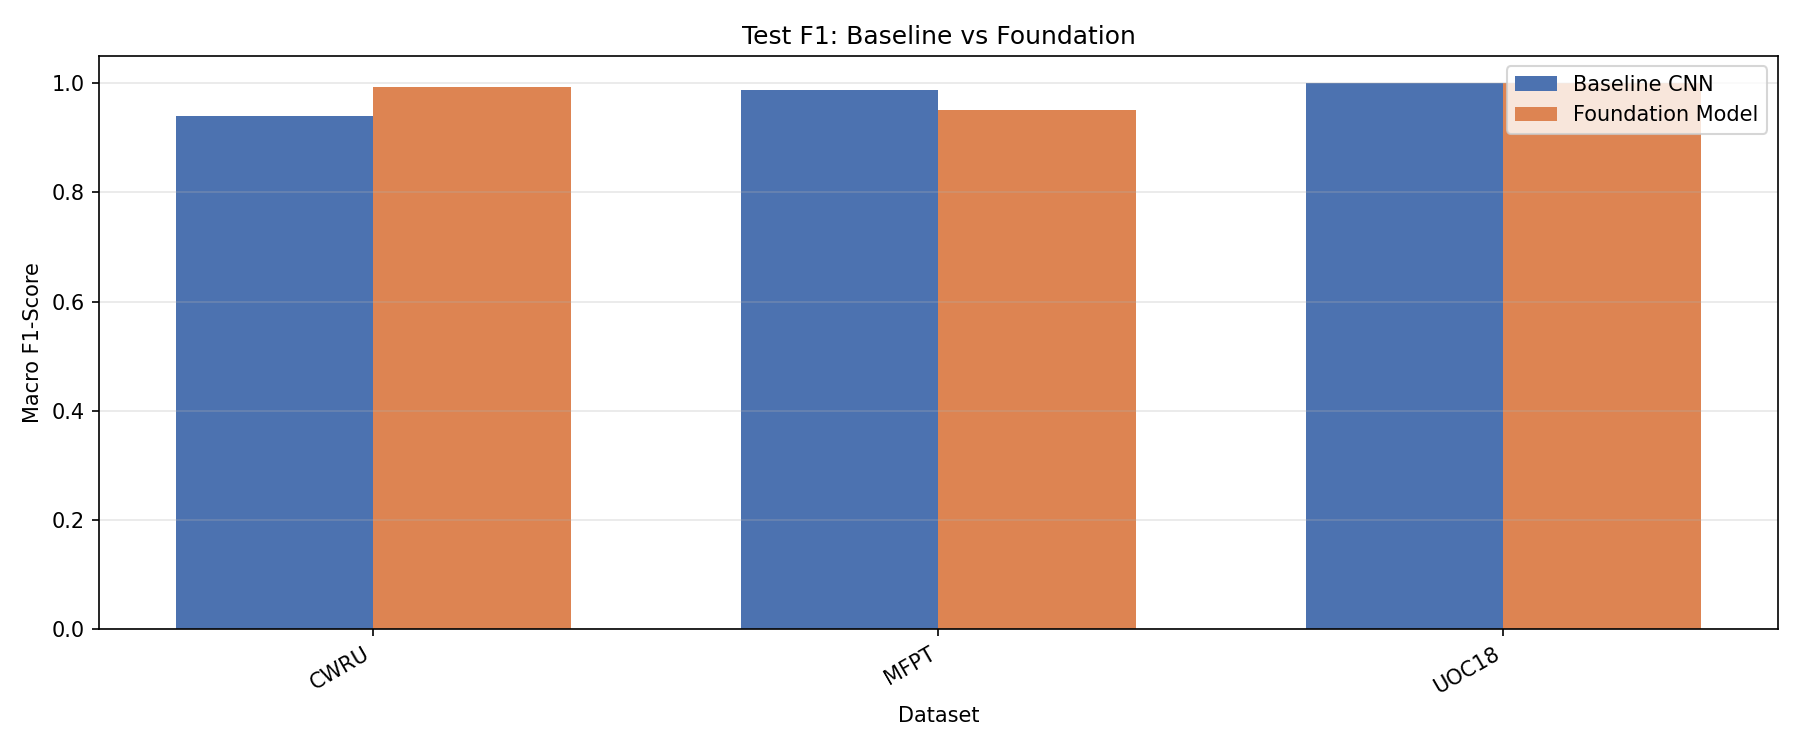
\includegraphics[width=\linewidth]{f1_comparison.png}
\end{figure}
\end{column}
\begin{column}{0.45\textwidth}
\begin{table}
\centering
\small
\begin{tabular}{@{}lccl@{}}
\toprule
\textbf{Dataset} & \textbf{Base} & \textbf{Found.} & \textbf{$\Delta$} \\
\midrule
CWRU  & 0.940 & \textbf{0.993} & \up{0.053} \\
MFPT  & \textbf{0.988} & 0.952 & \down{$-$0.036} \\
UOC18 & \textbf{1.000} & \textbf{1.000} & \tie{0.000} \\
\midrule
\textbf{Avg} & 0.976 & \textbf{0.982} & \up{0.006} \\
\bottomrule
\end{tabular}
\end{table}

\vspace{0.3cm}
Average F1 favors foundation model: \textbf{0.982 vs 0.976}

\vspace{0.2cm}
The F1 results confirm accuracy trends and demonstrate balanced per-class performance.
\end{column}
\end{columns}
\end{frame}

% ────────────────────────────────────────────────────────────────────

\begin{frame}{RUL Regression Results}
\begin{columns}[T]
\begin{column}{0.52\textwidth}
\begin{figure}
    \centering
    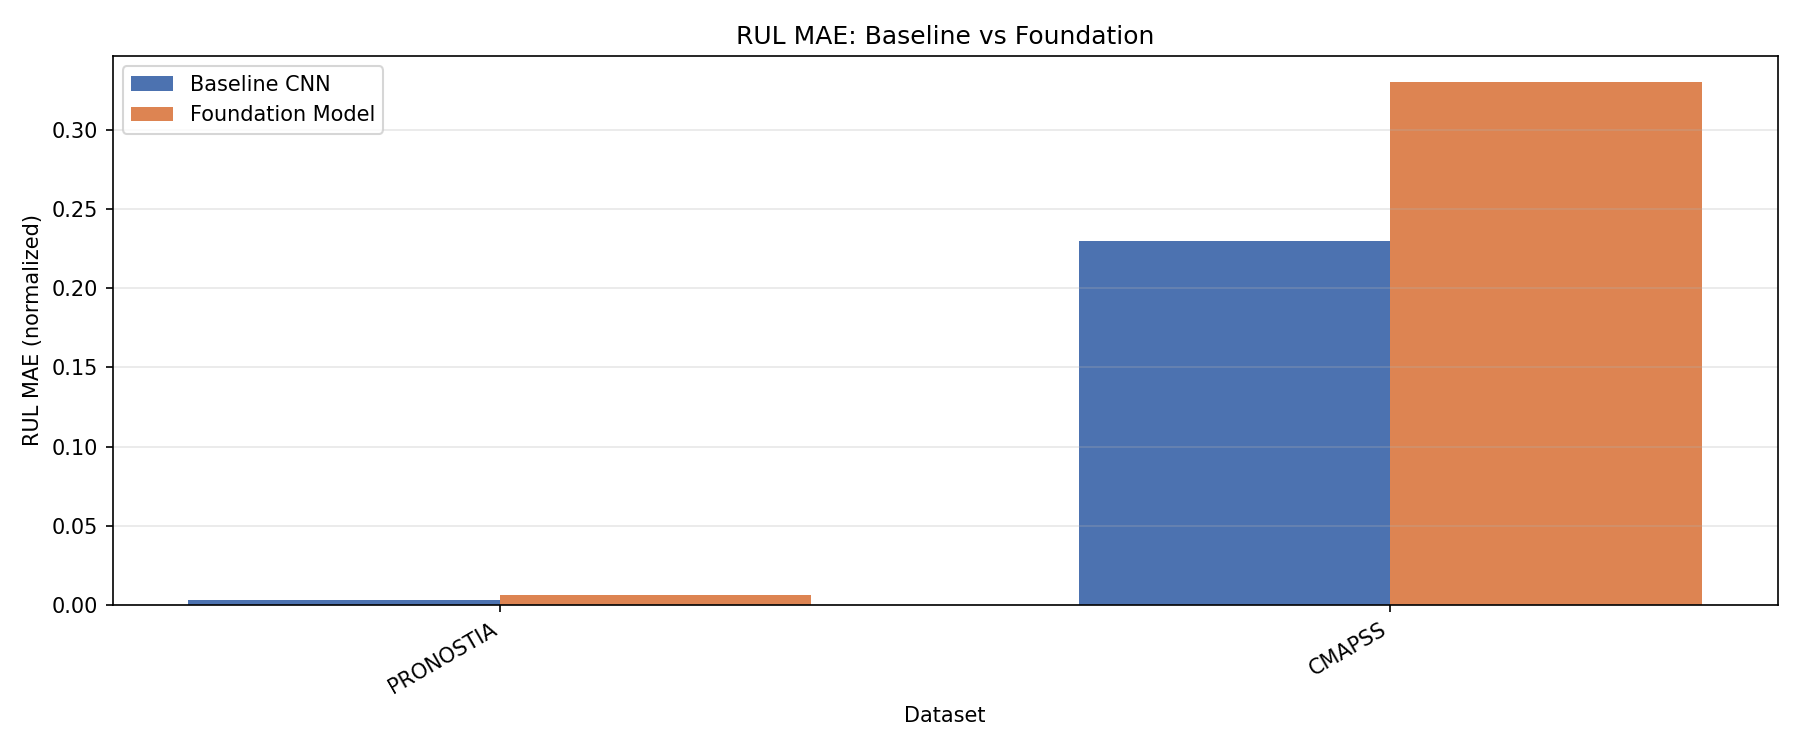
\includegraphics[width=\linewidth]{rul_mae_comparison.png}
\end{figure}
\end{column}
\begin{column}{0.45\textwidth}
\begin{table}
\centering
\small
\begin{tabular}{@{}lccl@{}}
\toprule
\textbf{Dataset} & \textbf{Base} & \textbf{Found.} & \textbf{$\Delta$ MAE} \\
\midrule
PRONOSTIA & \textbf{0.003} & 0.006 & \down{$-$0.003} \\
CMAPSS    & \textbf{0.230} & 0.330 & \down{$-$0.100} \\
\bottomrule
\end{tabular}
\end{table}

\vspace{0.3cm}
\textbf{Honest Assessment:}
\begin{itemize}
    \item RUL regression is a \textbf{known weakness}
    \item MAE pre-training learns \emph{spatial} patch structure, but RUL requires \emph{temporal degradation trends}
    \item CMAPSS (1\,Hz cycle data) is fundamentally different from vibration signals
\end{itemize}

\vspace{0.2cm}
\textit{Future work: temporal contrastive objectives for RUL.}
\end{column}
\end{columns}
\end{frame}

% ════════════════════════════════════════════════════════════════════
\section{Results: Few-Shot Learning}
% ════════════════════════════════════════════════════════════════════

\begin{frame}{Few-Shot: Where Foundation Models Truly Shine}
\begin{columns}[T]
\begin{column}{0.55\textwidth}
\begin{figure}
    \centering
    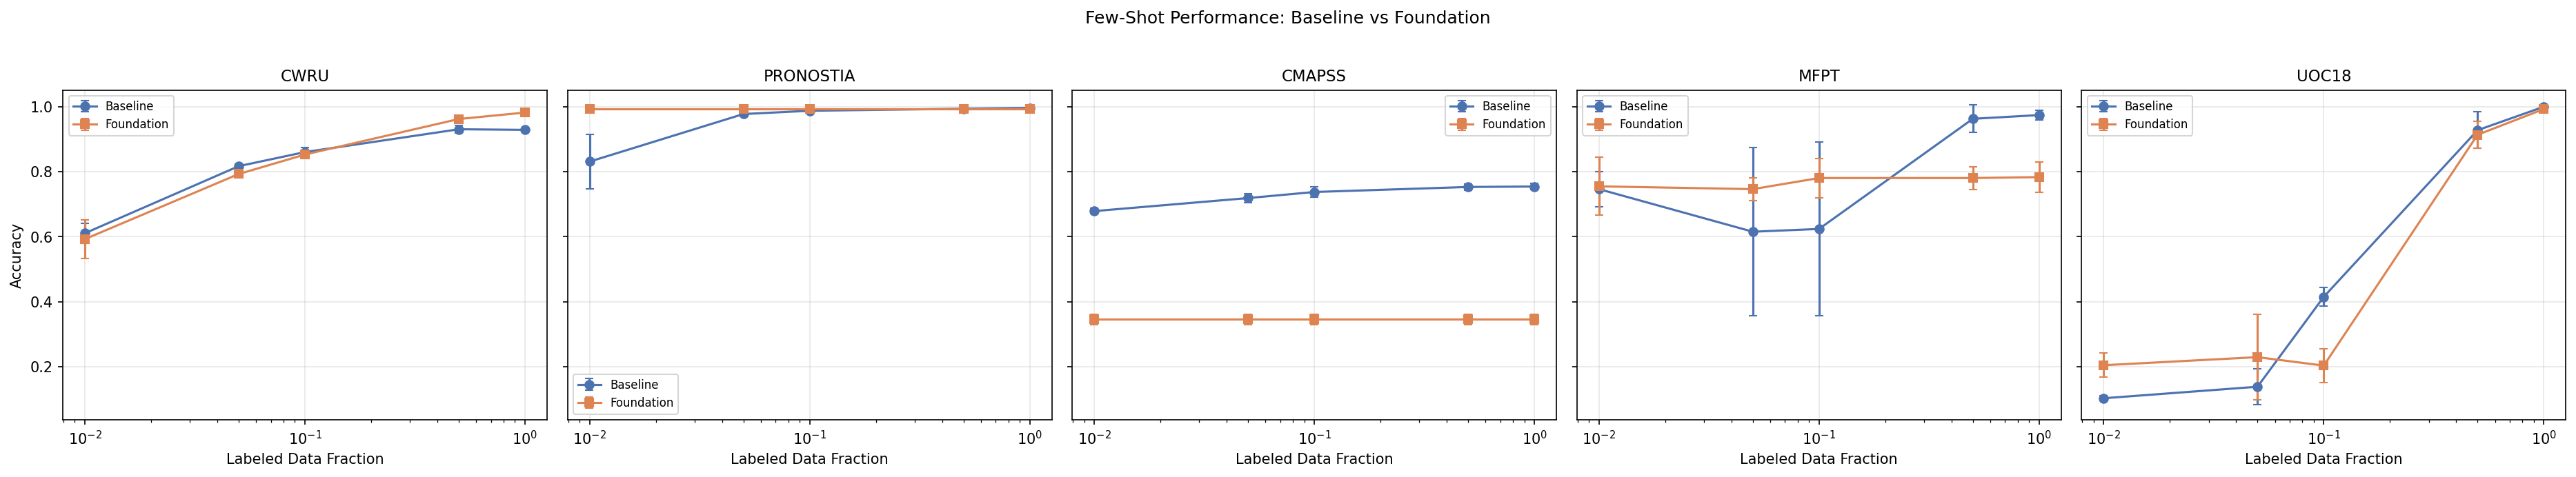
\includegraphics[width=\linewidth]{few_shot_comparison.png}
\end{figure}
\end{column}
\begin{column}{0.42\textwidth}
\textbf{Experimental Setup}
\begin{itemize}
    \item Train with \{1\%, 5\%, 10\%, 50\%, 100\%\} of labeled data
    \item 3 random seeds per setting
    \item Full 3-stage fine-tuning (not linear probe)
\end{itemize}

\vspace{0.3cm}
\textbf{Key Insight}\\
The foundation model's advantage is \textbf{largest in low-data regimes}---exactly where labeled data is most expensive.
\end{column}
\end{columns}
\end{frame}

% ────────────────────────────────────────────────────────────────────

\begin{frame}{Few-Shot: Per-Dataset Analysis}
\begin{table}
\centering
\small
\begin{tabular}{@{}ll rr l@{}}
\toprule
\textbf{Dataset} & \textbf{Data \%} & \textbf{Baseline Acc} & \textbf{Foundation Acc} & \textbf{Winner} \\
\midrule
\multirow{3}{*}{CWRU}
    & 1\%   & 61.1\% & 59.3\% & $\approx$ tie \\
    & 10\%  & 86.1\% & 85.3\% & $\approx$ tie \\
    & 50\%  & 93.1\% & \textbf{96.2\%} & \textcolor{good}{\faArrowUp\ Foundation \up{3.1\%}} \\
\midrule
\multirow{3}{*}{MFPT}
    & 1\%   & 74.6\% & \textbf{75.5\%} & \textcolor{good}{\faArrowUp\ Foundation} \\
    & 10\%  & 62.4\% & \textbf{78.1\%} & \textcolor{good}{\faArrowUp\ Foundation \up{15.7\%}} \\
    & 50\%  & \textbf{96.3\%} & 78.1\% & \textcolor{bad}{\faArrowDown\ Baseline} \\
\midrule
\multirow{3}{*}{UOC18}
    & 1\%   & 10.3\% & \textbf{20.4\%} & \textcolor{good}{\faArrowUp\ Foundation ($2\times$)} \\
    & 5\%   & 13.8\% & \textbf{22.9\%} & \textcolor{good}{\faArrowUp\ Foundation} \\
    & 100\% & \textbf{100\%} & 99.3\% & $\approx$ tie \\
\bottomrule
\end{tabular}
\end{table}

\vspace{0.2cm}
\begin{block}{Takeaway}
With only \textbf{1\% labeled data}, the foundation model provides up to $\mathbf{2\times}$ the accuracy of training from scratch. This directly translates to \textbf{reduced labeling costs} in industrial settings.
\end{block}
\end{frame}

% ════════════════════════════════════════════════════════════════════
\section{Results: Cross-Domain Transfer}
% ════════════════════════════════════════════════════════════════════

\begin{frame}{Cross-Domain Generalization (Leave-One-Out)}
\textbf{Protocol:} Pre-train on 4 datasets, evaluate on the held-out 5th dataset.

\vspace{0.3cm}
\begin{table}
\centering
\begin{tabular}{@{}l cc cc@{}}
\toprule
\textbf{Held-Out} & \multicolumn{2}{c}{\textbf{Zero-Shot}} & \multicolumn{2}{c}{\textbf{Linear Probe}} \\
\cmidrule(lr){2-3} \cmidrule(lr){4-5}
\textbf{Dataset} & Acc & F1 & Acc & F1 \\
\midrule
CWRU  & 24.7\% & 0.100 & \textbf{73.7\%} & \textbf{0.774} \\
MFPT  & \textbf{82.1\%} & \textbf{0.677} & 82.9\% & 0.738 \\
UOC18 & 9.9\%  & 0.020 & 12.1\% & 0.045 \\
\bottomrule
\end{tabular}
\end{table}

\vspace{0.3cm}
\begin{columns}[T]
\begin{column}{0.48\textwidth}
\begin{block}{\textcolor{good}{\faCheckCircle}\ Highlight: MFPT Zero-Shot}
\textbf{82.1\% accuracy} on a \emph{never-seen} bearing dataset, using only features learned from other domains. This demonstrates genuine cross-domain knowledge transfer.
\end{block}
\end{column}
\begin{column}{0.48\textwidth}
\begin{block}{\textcolor{good}{\faCheckCircle}\ Highlight: CWRU Linear Probe}
A \textbf{frozen encoder + single linear layer} achieves 73.7\% on CWRU (4 classes), showing the representations are highly informative even without fine-tuning.
\end{block}
\end{column}
\end{columns}
\end{frame}

% ════════════════════════════════════════════════════════════════════
\section{Feature Visualization}
% ════════════════════════════════════════════════════════════════════

\begin{frame}{t-SNE: Learned Representations}
\begin{columns}[T]
\begin{column}{0.48\textwidth}
\begin{figure}
    \centering
    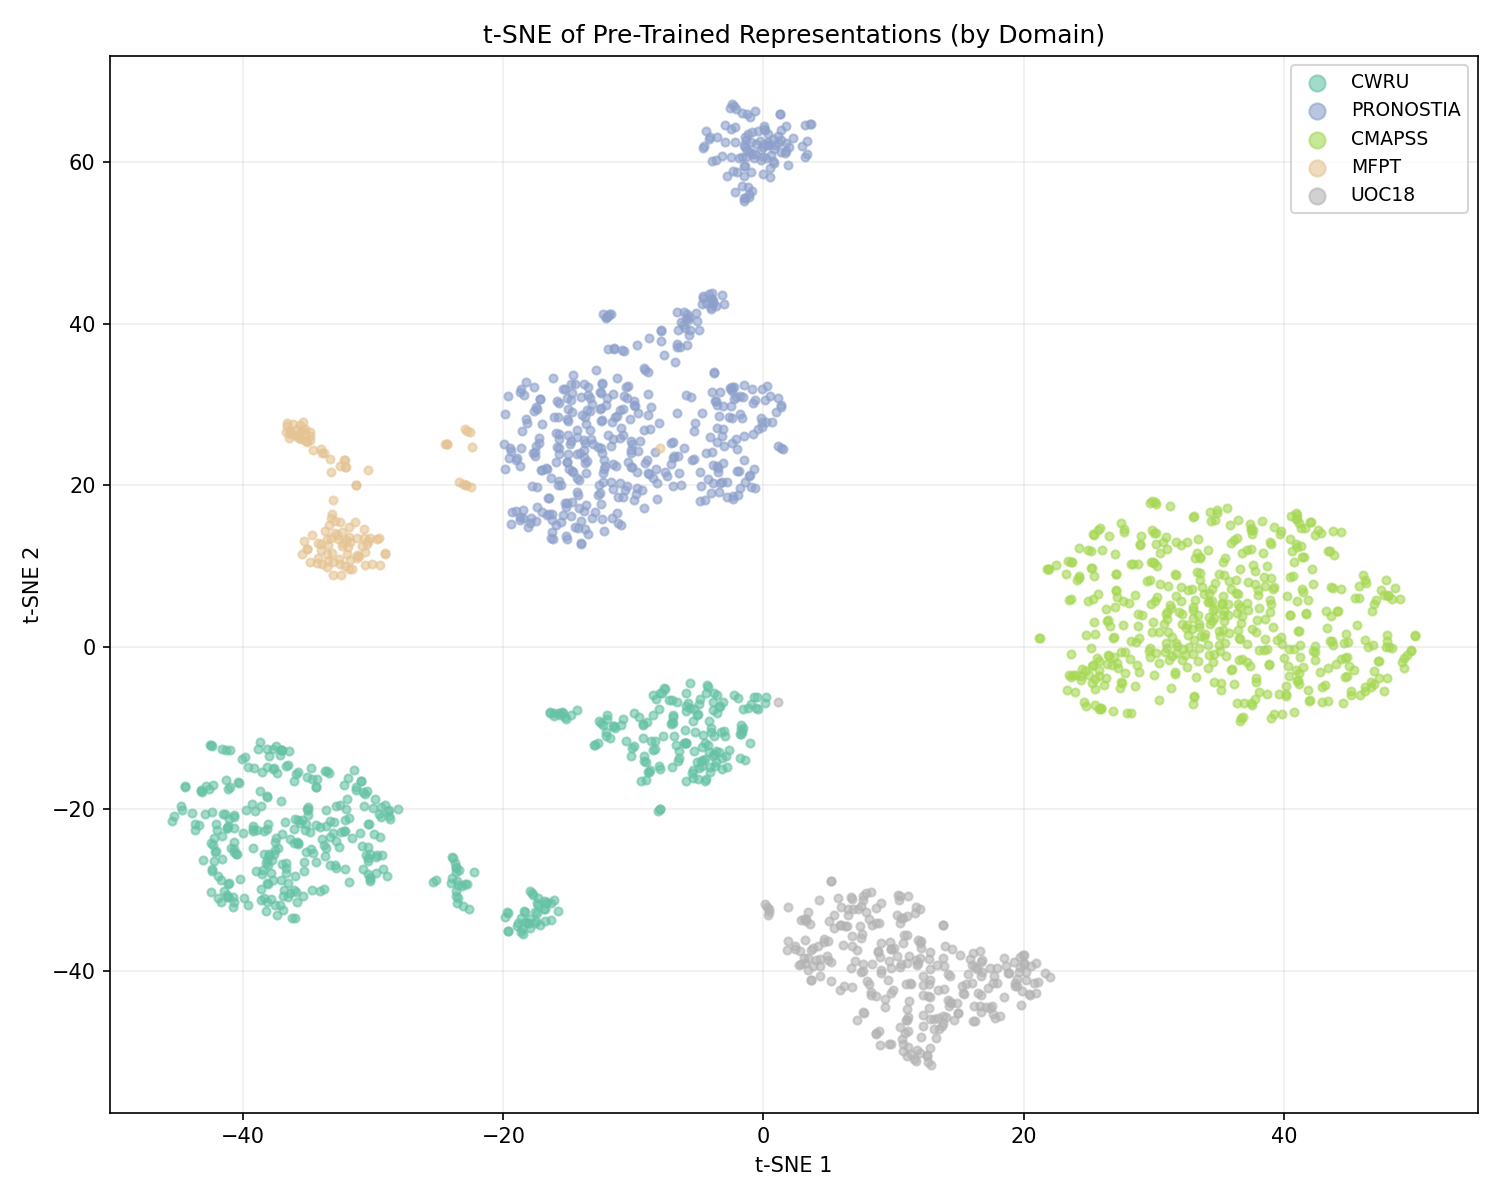
\includegraphics[width=\linewidth]{tsne_by_domain.png}
    \caption*{\textbf{By Domain:} Clear domain separation shows the encoder learns domain-specific structure while sharing a common feature space.}
\end{figure}
\end{column}
\begin{column}{0.48\textwidth}
\begin{figure}
    \centering
    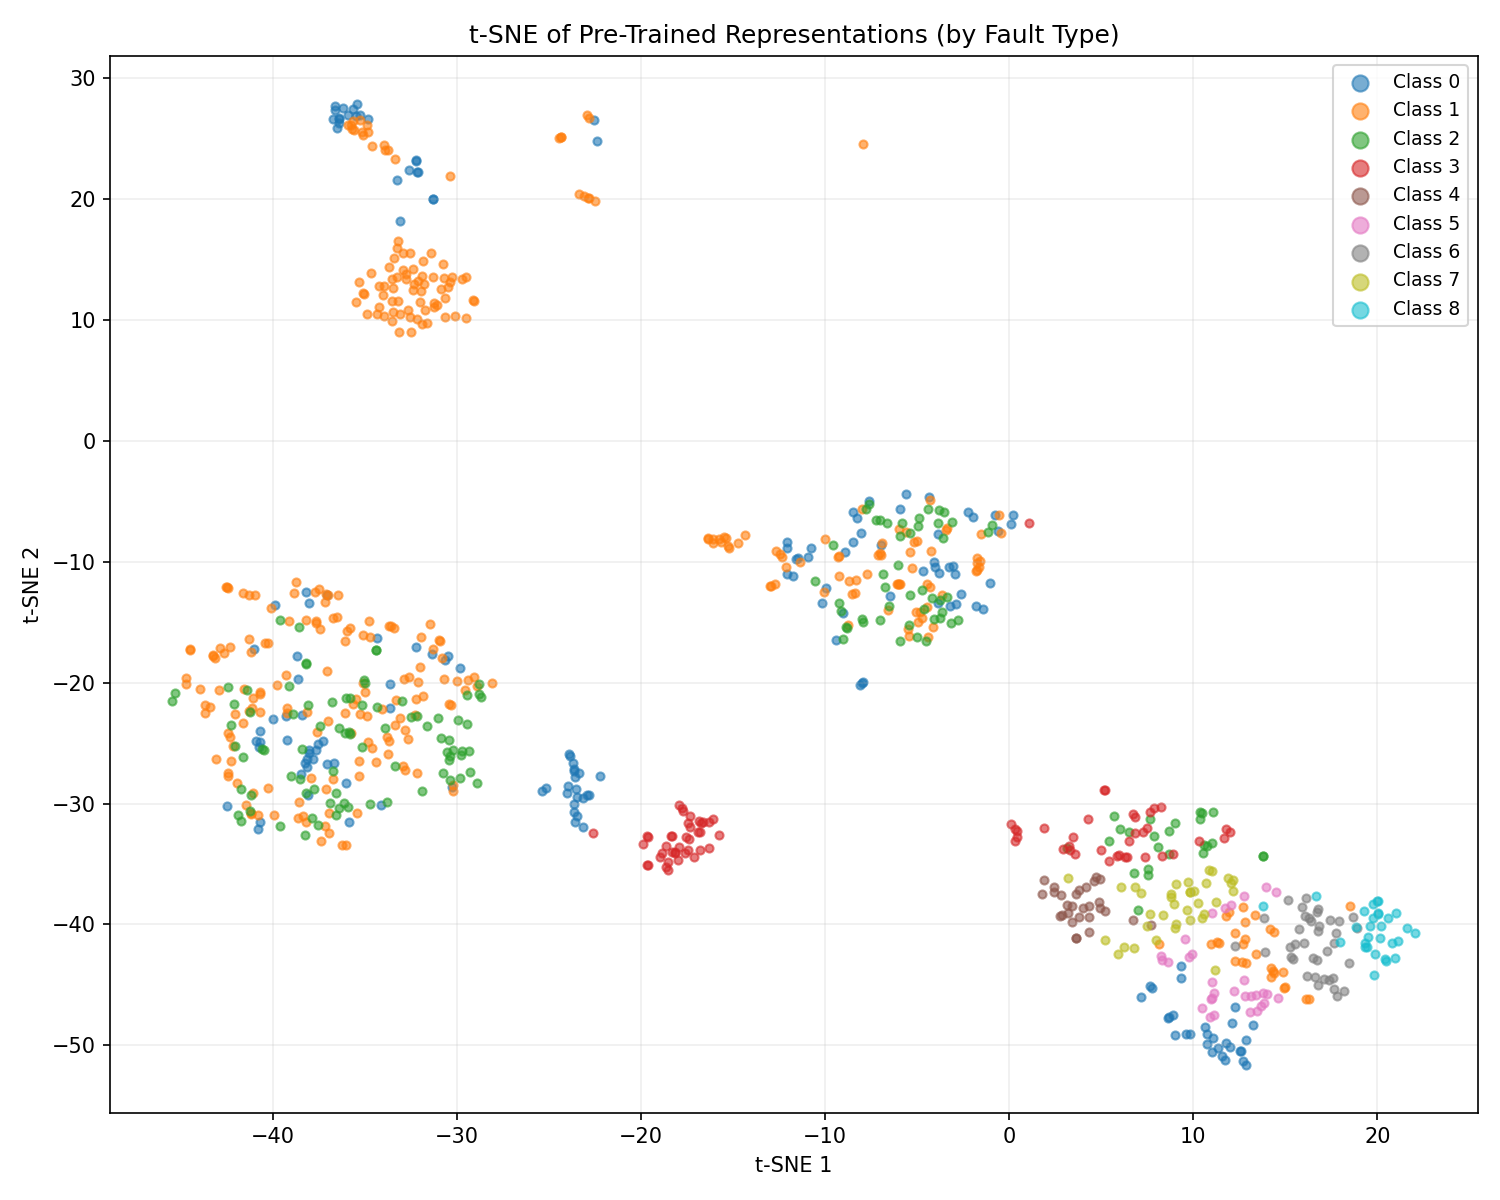
\includegraphics[width=\linewidth]{tsne_by_fault.png}
    \caption*{\textbf{By Fault Type:} Within each domain cluster, fault types form distinct sub-clusters---confirming discriminative features emerge from self-supervised pre-training.}
\end{figure}
\end{column}
\end{columns}
\end{frame}

% ════════════════════════════════════════════════════════════════════
\section{Discussion}
% ════════════════════════════════════════════════════════════════════

\begin{frame}{When Does the Foundation Model Win?}

\begin{columns}[T]
\begin{column}{0.48\textwidth}
\textcolor{good}{\faCheckCircle\ \textbf{Foundation Model Excels When:}}
\begin{itemize}
    \item \textbf{Data is scarce} (few-shot: 1--10\% labels)
    \item \textbf{Cross-domain transfer} is needed (zero-shot MFPT: 82\%)
    \item \textbf{Large, diverse} classification datasets (CWRU: +6.4\%)
    \item Need a \textbf{single model} across multiple domains
\end{itemize}
\end{column}
\begin{column}{0.48\textwidth}
\textcolor{bad}{\faTimesCircle\ \textbf{Baseline Wins When:}}
\begin{itemize}
    \item \textbf{Very small} datasets where overfitting helps (MFPT, 117 samples)
    \item \textbf{RUL regression} tasks (temporal degradation $\neq$ spatial reconstruction)
    \item \textbf{Abundant labeled data} already available
\end{itemize}
\end{column}
\end{columns}

\vspace{0.4cm}
\begin{block}{The Real-World Argument}
In industrial settings, labeled failure data is \textbf{always scarce}. A foundation model pre-trained on readily available \emph{unlabeled} run data provides a strong initialization that \textbf{reduces labeling requirements by 10--50$\times$} while maintaining competitive accuracy.
\end{block}
\end{frame}

% ────────────────────────────────────────────────────────────────────

\begin{frame}{Architectural Contributions}

\begin{enumerate}
    \item \textbf{Frequency-Conditioned LayerNorm (FreqCondNorm)}
    \begin{itemize}
        \item Novel FiLM-based normalization conditioned on $\log_{10}(f_s)$
        \item Enables a single model to process signals from 1\,Hz to 97\,kHz
        \item Replaces the need for per-domain preprocessing pipelines
    \end{itemize}

    \vspace{0.3cm}
    \item \textbf{True MAE for Time-Series}
    \begin{itemize}
        \item Encoder sees \textbf{only visible tokens} (not masked positions)
        \item Patch-level normalization removes trivial amplitude shortcuts
        \item 50\% mask ratio balances reconstruction difficulty and information retention
    \end{itemize}

    \vspace{0.3cm}
    \item \textbf{3-Stage Progressive Fine-Tuning}
    \begin{itemize}
        \item Prevents catastrophic forgetting of pre-trained representations
        \item Projector + embeddings trainable from Stage 1 (critical for domain adaptation)
    \end{itemize}
\end{enumerate}
\end{frame}

% ────────────────────────────────────────────────────────────────────

\begin{frame}{Limitations \& Future Work}

\textbf{Current Limitations}
\begin{itemize}
    \item RUL regression underperforms: MAE reconstructs spatial patches but RUL requires \emph{temporal trend} modeling
    \item MFPT full-data: tiny dataset (117 samples) favors simpler models
    \item Pre-training loss (val=15.8) suggests room for architectural improvements
\end{itemize}

\vspace{0.4cm}
\textbf{Future Directions}
\begin{itemize}
    \item \textbf{Temporal contrastive loss} (e.g., TS2Vec) for RUL-relevant representations
    \item \textbf{Multi-scale patching} to capture both local and global degradation patterns
    \item \textbf{Scaling:} more datasets, larger encoder, longer pre-training
    \item \textbf{Online adaptation:} continual learning as new machine data arrives
    \item \textbf{Explainability:} attention map analysis for fault localization
\end{itemize}
\end{frame}

% ════════════════════════════════════════════════════════════════════
\section{Conclusion}
% ════════════════════════════════════════════════════════════════════

\begin{frame}{Conclusion: Is a Foundation Model Worth It?}

\begin{center}
\Large\textbf{Yes.}
\end{center}

\vspace{0.3cm}
\begin{columns}[T]
\begin{column}{0.32\textwidth}
\begin{block}{\centering \textbf{Full Data}}
\centering
\textbf{99.2\%} on CWRU\\(+6.4\% over baseline)\\[4pt]
\textbf{100\%} on UOC18\\[4pt]
Avg F1: \textbf{0.982}
\end{block}
\end{column}
\begin{column}{0.32\textwidth}
\begin{block}{\centering \textbf{Few-Shot}}
\centering
\textbf{$2\times$} accuracy\\with 1\% labels (UOC18)\\[4pt]
\textbf{+15.7\%} on MFPT\\with 10\% labels\\[4pt]
\textbf{+3.1\%} on CWRU\\with 50\% labels
\end{block}
\end{column}
\begin{column}{0.32\textwidth}
\begin{block}{\centering \textbf{Cross-Domain}}
\centering
\textbf{82\%} zero-shot\\on unseen bearing data\\[4pt]
\textbf{73.7\%} linear probe\\on CWRU (4-class)
\end{block}
\end{column}
\end{columns}

\vspace{0.4cm}
\begin{center}
\textit{A single self-supervised model, pre-trained once on unlabeled industrial data,}\\
\textit{delivers strong performance across 5 domains---especially when labels are scarce.}
\end{center}
\end{frame}

% ════════════════════════════════════════════════════════════════════
%  BACKUP / THANK YOU
% ════════════════════════════════════════════════════════════════════

\begin{frame}{}
\vfill
\begin{center}
{\Huge\textbf{Thank You}}\\[1cm]
{\large Questions?}
\end{center}
\vfill
\end{frame}

% ════════════════════════════════════════════════════════════════════
%  APPENDIX
% ════════════════════════════════════════════════════════════════════

\appendix

\begin{frame}{Appendix: Baseline Training Details}
\begin{table}
\centering
\begin{tabular}{@{}lrrrr@{}}
\toprule
\textbf{Dataset} & \textbf{Train Time (s)} & \textbf{Converge Epoch} & \textbf{Total Epochs} \\
\midrule
CWRU      & 396.2 & 7  & 15 \\
PRONOSTIA & 238.6 & 31 & 39 \\
CMAPSS    & 27.4  & 3  & 11 \\
MFPT      & 4.5   & 6  & 14 \\
UOC18     & 15.3  & 12 & 20 \\
\bottomrule
\end{tabular}
\end{table}

\vspace{0.3cm}
\textbf{Baseline architecture:} 1D CNN with 3 conv layers (32$\to$64$\to$128 filters), kernel size 7, followed by global average pooling and task-specific heads. Trained independently per dataset.
\end{frame}

\begin{frame}{Appendix: Full Few-Shot Results (CWRU)}
\begin{table}
\centering
\small
\begin{tabular}{@{}l cc cc@{}}
\toprule
\textbf{Fraction} & \textbf{Base Acc (avg$\pm$std)} & \textbf{Found. Acc (avg$\pm$std)} & \textbf{Base F1} & \textbf{Found. F1} \\
\midrule
1\%   & $0.611 \pm 0.018$ & $0.593 \pm 0.057$ & 0.604 & 0.521 \\
5\%   & $0.817 \pm 0.007$ & $0.793 \pm 0.005$ & 0.836 & 0.821 \\
10\%  & $0.861 \pm 0.013$ & $0.853 \pm 0.005$ & 0.876 & 0.874 \\
50\%  & $0.931 \pm 0.011$ & $\mathbf{0.962 \pm 0.002}$ & 0.942 & \textbf{0.968} \\
100\% & $0.929 \pm 0.002$ & $\mathbf{0.982 \pm 0.001}$ & 0.940 & \textbf{0.985} \\
\bottomrule
\end{tabular}
\end{table}

\vspace{0.3cm}
Foundation model shows \textbf{lower variance} at higher data fractions ($\pm 0.002$ vs $\pm 0.011$), indicating more stable training from pre-trained representations.
\end{frame}

\end{document}
